\newif\ifglobal

%%%%%%%%%%%%%%%%%%%%%%%
%%% Compile to view %%%
%%%%%%%%%%%%%%%%%%%%%%%

%%%%%%%%%%%%%%%%%%%%%%%%%%%%%%%%%%%%%%%%%%%%%%%%%%%
%%% Readme:                                     %%%
%%% https://www.overleaf.com/read/bwdjvfjksvjy/ %%%
%%%%%%%%%%%%%%%%%%%%%%%%%%%%%%%%%%%%%%%%%%%%%%%%%%%

% >>> M?: marks a module setting number or important notice

% >>> M4: Set {./relative-path} to external files for this module <<<
\def \modulefiles {./22-I2S}
% To add an external file, use:
% (Replace '---' with actual filename)
% '\input{\modulefiles/tables/---.tex}' for tables
% '\includegraphics{\modulefiles/figures/---}' for figures
% '\subfile{\modulefiles/---}' for register files


% >>> M1: This module is in global project? <<<
% 'YES' - uncomment; 'NO' - comment out
\globaltrue

\ifglobal
    \documentclass[main\_\_CN.tex]{subfiles}

\else
    % Font "FandolSong-Regular" used by ctex does not have GSUB table.
    % It causes warnings that do not affect compilation and can be ignored.
    \PassOptionsToPackage{quiet}{fontspec}

    \documentclass[openany, 10pt]{book}

    % >>> M2: In ./00-shared/preamble-trm-module, also find
    %         settings for visibility of todo notes, watermark <<<
    \usepackage{preamble-trm-module}

    % Enable Chinese typesetting
    \usepackage{ctex}

    % >>> M3: Temporary labels in Chinese
    %         you can add your own labels there <<<
    \myexternaldocument{./00-shared/temp-labels-cn}

\fi %\ifglobal


\setcounter{secnumdepth}{4}


% >>> M5: If this module needs any updates in
% './00-shared/preamble-trm-module.sty'
% (include additional package, etc.), contact your module PM
% or create the file './00-shared/changelog.tex' make the
% necessary updates yourself and document them in this file <<<

% Make text left-aligned and allow latex to break pages naturally, comment out for full justification
\raggedright
\raggedbottom


\begin{document}


% Sets language into which pre-defined bits of text are translated
\selectlanguage{chinese}
\setchineseformatting


% Do not delete this block
\ifglobal
% Add the following front matter if
% this module is outside of global project
\else
    \InputIfFileExists{readme}{}{}
    \listoftodos
    {\let\clearpage\relax \listofdonetodos}
    \tableofcontents
    %\listoftables
    %\listoffigures
\fi


%%%%%%%%%%%%%%%%%%%%%%%%%
%%% TRM Module Begins %%%
%%%%%%%%%%%%%%%%%%%%%%%%%

\hypertarget{i2s}{}
\chapter{I2S 控制器 (I2S)}
\label{mod:i2s}

\section{概述}
I2S 总线为多媒体应用，尤其是数字音频应用提供了灵活的数据通信接口。ESP32 内置两个 I2S 接口，即 I2S0 和 I2S1。

I2S 标准总线定义了三种信号：时钟信号 BCK、声道选择信号 WS 和串行数据信号 SD。一个基本的 I2S 数据总线有一个主机和一个从机。主机和从机的角色在通信过程中保持不变。ESP32 的 I2S 模块包含独立的发送和接收声道，能够保证优良的通信性能。

\begin{figure}[H]
    \centering
    \fbox{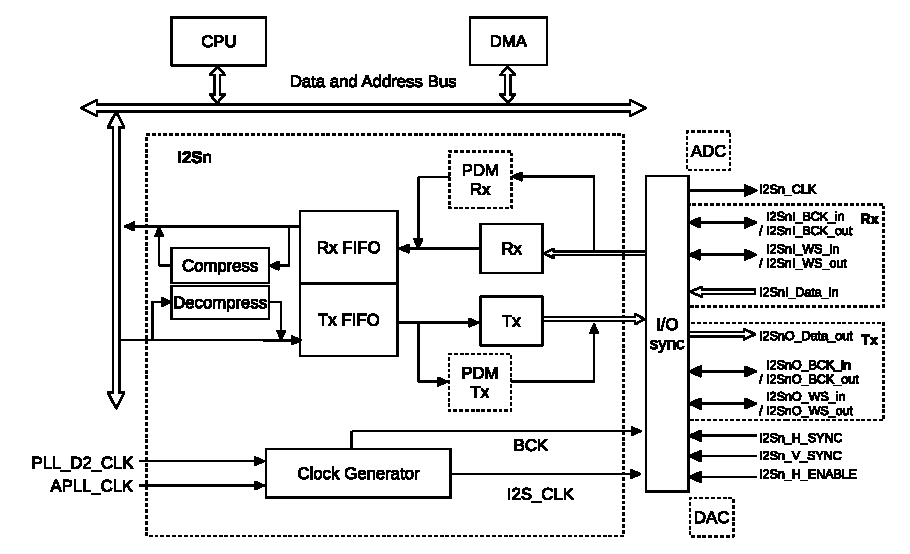
\includegraphics[width=0.9\textwidth]{./22-I2S/figures/i2s_arch}}
    \caption{I2S 系统框图}
    \label{Figure:i2s_arch}
\end{figure}

图 \ref{Figure:i2s_arch} 是 ESP32 I2S 模块的结构框图，图中 "\textcolor{red}{\it{n}}" 对应为 0 或 1，即 I2S0 或 I2S1。每个 I2S 模块包含一个独立的发送单元 (Tx) 和一个独立的接收单元 (Rx)。发送和接收单元各自有一组三线接口，分别为时钟线 BCK，声道选择线 WS 和串行数据线 SD。其中，发送单元的串行数据线固定为输出， 接收单元的串行数据线固定为接收。 发送单元和接收单元的时钟线和声道选择线均可配置为主机发送和从机接收。 在 LCD 模式下， 串行数据线扩展为并行数据总线。I2S 模块发送和接收单元各有一块宽 32 bit、深 64 bit 的 FIFO。此外，只有 I2S0 支持接收/发送 PDM 信号并且支持片上 DAC/ADC 模块。

图 \ref{Figure:i2s_arch} 右侧为 I2S 模块的信号总线。Rx 和 Tx 模块的信号命名规则为: I2S\textcolor{red}{\it{n}}A\_B\_C。其中 "\textcolor{red}{\it{n}}"为模块名，表示 I2S0 或 I2S1； "A"表示 I2S 模块的数据总线信号的方向，"I"表示输入，"O"表示输出；"B"表示信号功能；"C"表示该信号的方向，"in"表示该信号输入 I2S 模块，"out"表示该信号自 I2S 模块输出。 各信号总线的具体描述见表 \ref{table:I2S 信号总线描述}。除 I2S\textcolor{red}{\it{n}}\_CLK 信号外，其他信号均需要经过 GPIO 交换矩阵和 IO\_MUX 映射到芯片的管脚。I2S\textcolor{red}{\it{n}}\_CLK 信号需要经过 IO\_MUX 映射到芯片管脚。详情请参考章节 \hyperref[mod:iomuxgpio]{IO\_MUX 和 GPIO 交换矩阵}。

\begin{table}[H]
    \centering
    \caption{I2S 信号总线描述}
    \label{table:I2S 信号总线描述}
    \begin{tabular}{|p{3cm}|p{6cm}|p{6cm}| }
    \hline
    \rowcolor{lightgray}
    信号总线&信号方向&数据信号方向\\
    \hline
    I2S\textcolor{red}{\it{n}}I\_BCK\_in & 从机模式下，I2S 模块输入信号 &表示 I2S 模块接收数据\\
    \hline
    I2S\textcolor{red}{\it{n}}I\_BCK\_out& 主机模式下，I2S 模块输出信号& 表示 I2S 模块接收数据\\
    \hline
    I2S\textcolor{red}{\it{n}}I\_WS\_in & 从机模式下，I2S 模块输入信号& 表示 I2S 模块接收数据\\
    \hline
    I2S\textcolor{red}{\it{n}}I\_WS\_out&	主机模式下，I2S 模块输出信号& 表示 I2S 模块接收数据\\\hline
     \multirow{3}*{I2S\textcolor{red}{\it{n}}I\_Data\_in$^1$}& \multirow{3}*{I2S 模块输入信号}& I2S 模式下， I2S\textcolor{red}{\it{n}}I\_Data\_in[15] 为 I2S 的串行数据总线，LCD 模式下，可以根据需要配置数据总线的宽度\\\hline
    \multirow{3}*{I2S\textcolor{red}{\it{n}}O\_Data\_out$^1$} & \multirow{3}*{I2S 模块输出信号}& I2S 模式下，
    I2S\textcolor{red}{\it{n}}O\_Data\_out[23] 为 I2S 的串行数据总线，LCD 模式下，可以根据需要配置数据总线的宽度\\\hline
    I2S\textcolor{red}{\it{n}}O\_BCK\_in&	从机模式下，I2S 模块输入信号&表示 I2S 模块发送数据\\\hline
    I2S\textcolor{red}{\it{n}}O\_BCK\_out& 主机模式下，I2S 模块输出信号&表示 I2S 模块发送数据\\\hline
    I2S\textcolor{red}{\it{n}}O\_WS\_in& 从机模式下，I2S 模块输入信号&表示 I2S 模块发送数据\\\hline
    I2S\textcolor{red}{\it{n}}O\_WS\_out&	主机模式下，I2S 模块输出信号&表示 I2S 模块发送数据\\\hline
    I2S\textcolor{red}{\it{n}}\_CLK$^2$& I2S 模块输出信号&作为外部芯片的时钟源\\\hline
    I2S\textcolor{red}{\it{n}}\_H\_SYNC&\multirow{3}*{Camera 模式下，I2S 模块输入信号}&\multirow{3}*{ 来自 Camera 的信号 }\\
    \cline{1-1}
    I2S\textcolor{red}{\it{n}}\_V\_SYNC&&\\
    \cline{1-1}
    I2S\textcolor{red}{\it{n}}\_H\_ENABLE	&&\\
    \hline
    \end{tabular}
\end{table}
\vspace{-0.5em}
\begin{tiplisting}
\vspace{-2em}
\begin{enumerate}
    \item 假设 I2S 输入/输出信号位宽为 \textcolor{red}{\it{N}} 比特，那么 I2S 模块输入信号应配置为 I2S\textcolor{red}{\it{n}}I\_Data\_in[\textcolor{red}{\it{N}}-1:0]，I2S  模块输出信号应配置为 I2S\textcolor{red}{\it{n}}O\_Data\_out[23:23-\textcolor{red}{\it{N}}+1]。通常对输入信号 \textcolor{red}{\it{N}}=8 或 16，对输出信号 \textcolor{red}{\it{N}}=8，16 或 24（I2S1 不包含 24 bit 模式）。
    \item I2S\textcolor{red}{\it{n}}\_CLK 仅能映射至 GPIO0、U0RXD (GPIO3) 或 U0TXD (GPIO1) 管脚，选择 CLK\_OUT1、CLK\_OUT2 或 CLK\_OUT3 功能。更多信息见表 \ref{table:iomux_pads}：\textit{\nameref{table:iomux_pads}}。
\end{enumerate}
\end{tiplisting}

\section{主要特性}
I2S 模式
\begin{itemize}
    \item 可配置高精度输出时钟；
    \item 支持全双工和半双工收发数据；
    \item 支持多种音频标准；
    \item 内嵌 A 律压缩/解压缩模块；
    \item 可配置时钟；
    \item 支持 PDM 信号输入输出；
    \item 收发数据模式可配置。
\end{itemize}

LCD 模式
\begin{itemize}
    \item 支持外接 LCD；
    \item 支持外接 Camera；
    \item 支持多种 LCD 模式；
    \item 支持连接片上 DAC/ADC 模式。
\end{itemize}

I2S 中断
\begin{itemize}
    \item I2S 接口中断；
    \item I2S DMA 接口中断。
\end{itemize}

\section{I2S 模块时钟}\label{The Clock of I2S Module}
I2S\textcolor{red}{\it{n}}\_CLK 作为 I2S 模块的主时钟，是由 160 MHz 时钟 PLL\_F160M\_CLK 或者可配置的模拟 PLL 输出时钟 APLL\_CLK 进行分频获得。I2S 模块的串行时钟 BCK 再由 I2S\textcolor{red}{\it{n}}\_CLK 分频获得，如图 \ref{Figure:i2s_clk} 所示。寄存器 I2S\_CLKM\_CONF\_REG 中 I2S\_CLKA\_ENA 比特用于选择 PLL\_F160M\_CLK 还是 APLL\_CLK 作为 I2S\textcolor{red}{\it{n}} 的时钟源，默认使用 PLL\_F160M\_CLK 作为 I2S\textcolor{red}{\it{n}} 的时钟源。

{\bfseries 注意：}
\begin{itemize}
\item 在使用 PLL\_F160M\_CLK 作为时钟源时， 不建议使用小数分频功能。需要获得更高精度的 I2S\textcolor{red}{\it{n}}\_CLK 和 BCK 时，要使用 APLL\_CLK 作为时钟源，详情请参考章节\hyperref[mod:resclk]{复位和时钟}。
\item 当 ESP32 I2S 作为从机时，主机必须使用 ESP32 的 I2S\textcolor{red}{\it{n}}\_CLK 作为主 时钟， 同时 $f_{\textrm{i2s}}$ >= 8 * $f_{\textrm{BCK}}$。
\end{itemize}

\begin{figure}[H]
    \centering
    \fbox{
\includegraphics[width=0.6\textwidth]{./22-I2S/figures/i2s_clk}}
    \caption{I2S 时钟}
    \label{Figure:i2s_clk}
\end{figure}

I2S\textcolor{red}{\it{n}}\_CLK 的频率 $f_{\textrm{i2s}}$ 与分频器时钟源频率 $f_{\textrm{pll}}$ 间的关系如下：
$$f_{\textrm{i2s}}=\frac{f_{\textrm{pll}}}{\textrm{N} + \frac{\textrm{b}}{\textrm{a}}}$$
其中，N>=2，N 对应 I2S\_CLKM\_CONF\_REG 寄存器中的 I2S\_CLKM\_DIV\_NUM[7:0] 位，b 为 I2S\_CLKM\_DIV\_B[5:0] 位，a 为 I2S\_CLKM\_DIV\_A[5:0] 位。

在主机模式下，I2S 模块的串行时钟 BCK 由 I2S\textcolor{red}{\it{n}}\_CLK 分频获得。即：
$$f_{\textrm{BCK}} = \frac{f_{\textrm{i2s}}}{\textrm{M}}$$
其中，M>=2，在主机发送模式下， M 为寄存器 I2S\_SAMPLE\_RATE\_CONF\_REG 的 I2S\_TX\_BCK\_DIV\_NUM[5:0] 位，在主机接收模式下， M 为寄存器 I2S\_SAMPLE\_RATE\_CONF\_REG 的 I2S\_RX\_BCK\_DIV\_NUM[5:0] 位。

\section{I2S 模式}

ESP32 I2S 模块内置数据 A 律压缩/解压缩模块，用于对接收到的音频数据进行 A 律缩/解压缩操作。如果要使用 A 律缩/解压缩模块，需要将 I2S\_CONF1\_REG 寄存器的 RX\_PCM\_BYPASS 比特和 TX\_PCM\_BYPASS 比特清零。

\subsection{支持的音频标准}

I2S 模式下，BCK 为串行时钟；WS 为通道选择信号，用于表示左右声道的切换；SD 为串行数据信号，传输音频数据。WS 信号和 SD 信号在 BCK 的下降沿发生变化，并在 BCK 的上升沿采样 SD 信号。如果将寄存器 I2S\_CONF\_REG 的 I2S\_RX\_RIGHT\_FIRST 比特和 I2S\_TX\_RIGHT\_FIRST 比特都置 1，表示 I2S 模块首先接收和发送的是右声道数据，否则为首先接收和发送的是左声道数据。

\subsubsection{Philips 标准}\label{section:Philips Standard}

\begin{figure}[H]
    \centering
    \fbox{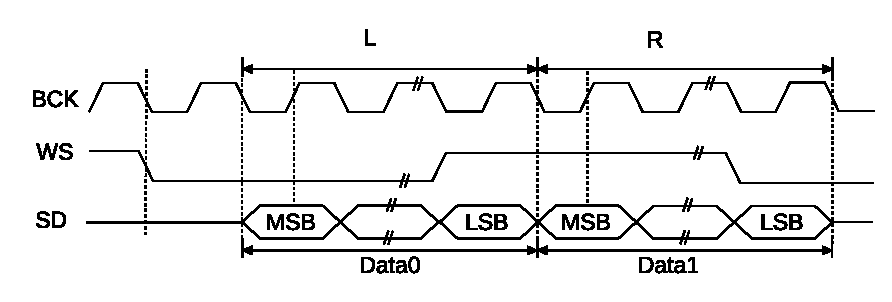
\includegraphics[width=0.6\textwidth]{./22-I2S/figures/i2s_phillips_standard}}
    \caption{Philips 标准}
    \label{Figure:i2s_phillips_standard}
\end{figure}

如图 \ref{Figure:i2s_phillips_standard} 所示，在 Philips 标准下，在 BCK 的下降沿，WS 信号先于 SD 信号一个 BCK 时钟周期开始变化，即 WS 信号从当前通道数据的第一个位之前的一个时钟开始有效，并在当前通道数据发送结束前一个BCK 时钟周期变化。SD 信号线首先传输音频数据的最高有效位。如果分别将寄存器 I2S\_CONF\_REG 的 I2S\_RX\_MSB\_SHIFT 比特和 I2S\_TX\_MSB\_SHIFT 比特置 1，I2S 模块接收数据和发送数据将使用 Philips 标准。

\subsubsection{MSB 对齐标准}

\begin{figure}[H]
    \centering
    \fbox{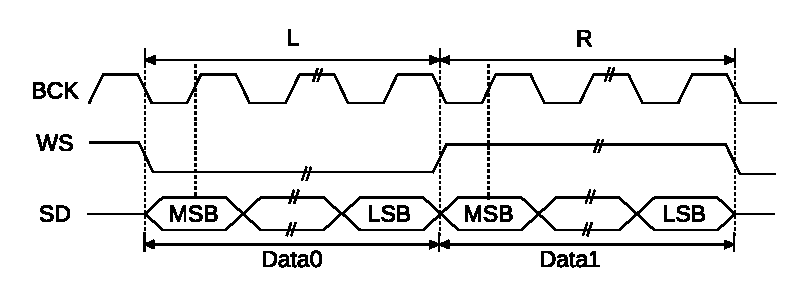
\includegraphics[width=0.6\textwidth]{./22-I2S/figures/i2s_MSB_32_mode}}
    \caption{MSB 对齐标准}
    \label{Figure:i2s_MSB_32_mode}
\end{figure}

如图 \ref{Figure:i2s_MSB_32_mode} 所示，MSB 对齐标准下，在 BCK 下降沿，WS 信号和 SD 信号同时变化。WS 持续到当前通道数据发
送结束，SD 信号线上首先传输音频数据的最高位。如果寄存器 I2S\_CONF\_REG 的 I2S\_RX\_MSB\_SHIFT 比特和 I2S\_TX\_MSB\_SHIFT 比特清零， 则 I2S 模块接收数据和发送数据将使用 MSB 对齐标准。

\subsubsection{PCM 标准}

\begin{figure}[H]
    \centering
    \fbox{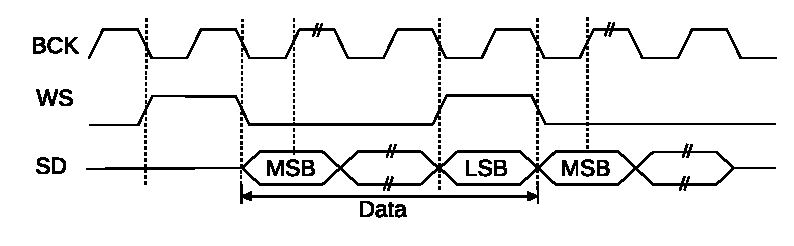
\includegraphics[width=0.6\textwidth]{./22-I2S/figures/i2s_pcm_mode}}
    \caption{PCM 标准}
    \label{Figure:i2s_pcm_mode}
\end{figure}

如图 \ref{Figure:i2s_pcm_mode} 所示，在 PCM 标准的短帧同步模式下，在 BCK 的下降沿，WS 信号先于 SD 信号一个 BCK 时钟周期开始变化，即 WS 信号从当前通道数据的第一个位之前的一个时钟开始有效，并持续 1 个 BCK 时钟周期。SD 信号线上首先传输音频数据的最高位。如果将寄存器 I2S\_CONF\_REG 的 I2S\_RX\_SHORT\_SYNC 比特和 I2S\_TX\_SHORT\_SYNC 比特置 1，那么 I2S 模块接收数据和发送数据将使用短帧同步模式。

\subsection{模块复位}
寄存器 I2S\_CONF\_REG 中的低四个比特为 I2S\_TX\_RESET 比特、 I2S\_RX\_RESET 比特、 I2S\_TX\_FIFO\_RESET 比特和 I2S\_RX\_FIFO\_RESET 比特， 分别表示对接收模块、发送模块和其对应的 FIFO 进行复位。完成一次复位操作需要先将对应比特置 1，然后清零。

\subsection{FIFO 操作}
I2S 一次 FIFO 操作， 写入/读取数据包长度为 32 位。 数据包格式由寄存器配置。 由图 \ref{Figure:i2s_arch} 可知， 待发送数据和接收到的数据，都要先写入 FIFO， 然后再读出。读写 FIFO 的方式有两种，一种是使用 CPU 直接进行读写，另一种是使用 DMA 控制器进行读写。

一般情况下 I2S\_FIFO\_CONF\_REG 寄存器的 I2S\_RX\_FIFO\_MOD\_FORCE\_EN 比特和 I2S\_TX\_FIFO\_MOD\_FORCE\_EN 比特均需要置为 1。I2S\_TX\_DATA\_NUM[5:0] 比特和 I2S\_RX\_DATA\_NUM[5:0] 比特用于控制 FIFO 缓冲发送数据和接收数据的长度。硬件自动检查 FIFO 缓存的接收数据长度 RX\_LEN 和发送数据长度 TX\_LEN。

当 RX\_LEN > I2S\_RX\_DATA\_NUM[5:0] 时，表示 FIFO 缓存的接收数据已经达到设定阈值，需要及时取走。当 TX\_LEN < I2S\_TX\_DATA\_NUM[5:0] 时，表示 FIFO 缓存的发送数据还未达到设定阈值，可以继续向 FIFO 中填充数据。

\subsection{发送数据}\label{TXCHAN}

ESP32 I2S 发送数据分为三个阶段：
\begin{itemize}
    \item 第一阶段从内存中读出数据并写入 FIFO；
    \item 第二阶段将待发送数据从 FIFO 中读出；
    \item  第三阶段， 在 I2S 模式下，将待发送数据转换为串行数据流输出；在 LCD 模式下，将待发送数据转换为位宽固定的并行数据流输出。
\end{itemize}

\begin{figure}[H]
    \centering
    \fbox{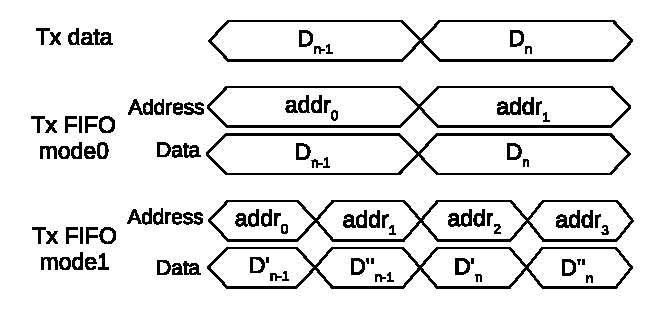
\includegraphics[width=0.6\textwidth]{./22-I2S/figures/i2s_tx_fifo_mode}}
    \caption{发送 FIFO 数据模式}
    \label{Figure:i2s_tx_fifo_mode}
\end{figure}

\begin{table}[H]
    \centering
    \caption{寄存器配置}
    \label{table:寄存器配置}
    \begin{tabular}{|p{5cm}|p{5cm}|p{5cm}| }
    \rowcolor{lightgray}
    \hline
    &I2S\_TX\_FIFO\_MOD[2:0]&描述\\\hline
    \multirow{3}*{Tx FIFO mode0} & 0 & 16 位双通道数据\\
    \cline{2-3}
    & 2 & 32 位双通道数据\\
    \cline{2-3}
    & 3 & 32 位单通道数据\\\hline
    Tx FIFO mode1    & 1 & 16 位单通道数据\\\hline
    \end{tabular}
\end{table}

在第一阶段，待发送数据写入 FIFO 的模式有两种。Tx FIFO mode0 条件下，待发送数据 Tx data 按时间先后被直接写入 FIFO；Tx FIFO mode1 条件下，待发送数据被分成高 16 比特和低 16 比特，重新组合后再写入 FIFO, 如图 \ref{Figure:i2s_tx_fifo_mode} 所示, 对应寄存器如表 \ref{table:寄存器配置} 所示。 $D^{'}_{n}$ 由 $D_{n}$ 的高 16 比特和 16 个 0 组成，$D^{''}_{n}$ 由 $D_{n}$ 的低 16 比特和 16 个 0 组成，即：$D^{'}_{n} = \{D_{n}[31:16],16'h0\}$， $D^{''}_{n} = \{D_{n}[15:0],16'h0\}$。

在第二阶段，系统会按照相关寄存器配置将待发送数据从 FIFO 读出。从 FIFO 读出数据的模式与\\
I2S\_TX\_FIFO\_MOD[2.0] 和 I2S\_TX\_CHAN\_MOD[2:0] 的取值有关。I2S\_TX\_FIFO\_MOD[2.0] 决定数据是 16 位还是 32 位；I2S\_TX\_CHAN\_MOD[2:0] 决定待发送数据的格式，如表 \ref{table:发送通道模式} 所示。

\begin{table}[H]
    \centering
    \caption{发送通道模式}
    \label{table:发送通道模式}
    \begin{tabular}{|p{5cm}|p{10cm}|}
    \hline
    \rowcolor{lightgray}
    I2S\_TX\_CHAN\_MOD[2:0]&描述\\ \hline
    0 & 双声道模式\\\hline
    \multirow{3}*{1} & 单声道模式\\
        &I2S\_TX\_MSB\_RIGHT=0 时，左声道和右声道数据均为左声道数据。\\
        &I2S\_TX\_MSB\_RIGHT=1 时，左声道和右声道数据均为右声道数据。\\\hline
    \multirow{3}*{2} & 单声道模式\\
        &I2S\_TX\_MSB\_RIGHT=0 时，左声道和右声道数据均为右声道数据。\\
        &I2S\_TX\_MSB\_RIGHT=1 时，左声道和右声道数据均为左声道数据。\\\hline
    \multirow{3}*{3} & 单声道模式\\
        &I2S\_TX\_MSB\_RIGHT=0 时，左声道数据为常数 REG[31:0]。\\
        &I2S\_TX\_MSB\_RIGHT=1 时，右声道数据为常数 REG[31:0]。\\
    \hline
    \multirow{3}*{4} & 单声道模式\\
        &I2S\_TX\_MSB\_RIGHT=0时，右声道数据为常数 REG[31:0]。\\
        &I2S\_TX\_MSB\_RIGHT=1时，左声道数据为常数 REG[31:0]。\\
    \hline
    \end{tabular}
\end{table}

其中 REG[31:0] 为寄存器 I2S\_CONF\_SINGLE\_DATA\_REG[31:0] 的值。

第三阶段输出由 I2S 的模式和寄存 器I2S\_SAMPLE\_RATE\_CONF\_REG 的 I2S\_TX\_BITS\_MOD[5:0] 比特决定。

\subsection{接收数据}\label{RXCHAN}

ESP32 I2S 接收数据也分为三个阶段：
\begin{itemize}
\item 第一阶段，在 I2S 模式下，输入的串行比特流数据会被以声道属性转换成宽度为 64 位的并行数据流；在 LCD 模式下，输入的位宽固定的并行数据流会被扩展成宽度为 64 位的并行数据流；
\item 第二阶段将待接收的数据写入 FIFO；
\item 第三阶段将待接收的数据从 FIFO 中读出，并写入内存。
\end{itemize}

在第一阶段，接收模块按 I2S\textcolor{red}{\it{n}}I\_WS\_out（或 I2S\textcolor{red}{\it{n}}I\_WS\_in） 信号电平的高低，将接收到数据流扩展成高电平对应 32 位和低电平对应 32 位的并行数据流，不足的补 0。寄存器 I2S\_CONF\_REG 的 I2S\_RX\_MSB\_RIGHT 比特用于确定扩展后数据的排列方式。

\begin{figure}[H]
    \centering
    \fbox{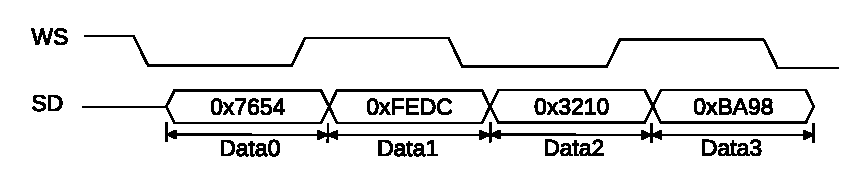
\includegraphics[width=0.7\textwidth]{./22-I2S/figures/i2s_rx_example}}
    \caption{第一阶段接收数据}
    \label{Figure:i2s_rx_example}
\end{figure}

例如，如图 \ref{Figure:i2s_rx_example} 所示， 如果串行数据宽度为 16 位，当 I2S\_RX\_RIGHT\_FIRST = 1 时，那么数据 Data0 将会被丢弃，I2S 将从 Data1 开始接收数据；此时若 I2S\_RX\_MSB\_RIGHT = 1， 那么第一阶段数据为 $\{0xFEDC0000,0x32100000\}$，若 I2S\_RX\_MSB\_RIGHT = 0，那么第一阶段数据为 $\{0x32100000,0xFEDC0000\}$。当 I2S\_RX\_RIGHT\_FIRST = 0 时，I2S 将从 Data0 开始接收数据；如果 I2S\_RX\_MSB\_RIGHT = 1，那么第一阶段数据为 $\{0xFEDC0000,0x76540000\}$，如果 I2S\_RX\_MSB\_RIGHT = 0，那么第一阶段数据为 $\{0x76540000,0xFEDC0000\}$。

在第二阶段，将接收模块接收到的数据写入 FIFO。 接收数据写入 FIFO 的模式共有四种，对应 I2S\_RX\_FIFO\_MOD[2:0] 比特取值，如表 \ref{table:接收数据写入FIFO模式和对应寄存器配置} 和图 \ref{Figure:i2s_rx_fifo_mode} 所示。

\begin{table}[H]
    \centering
    \caption{接收数据写入 FIFO 模式和对应寄存器配置}
    \label{table:接收数据写入FIFO模式和对应寄存器配置}
    \begin{tabular}{|p{7cm}|p{8cm}|}
    \hline
    \rowcolor{lightgray}
    I2S\_RX\_FIFO\_MOD[2:0]	&数据格式\\\hline
    0&	16 位双通道数据\\\hline
    1&	16 位单通道数据\\\hline
    2&	32 位双通道数据\\\hline
    3&	32 位单通道数据\\\hline
    \end{tabular}
\end{table}

\begin{figure}[H]
    \centering
    \fbox{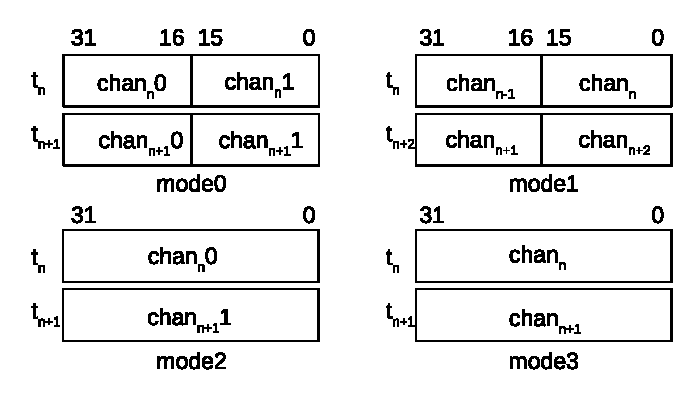
\includegraphics[width=0.6\textwidth]{./22-I2S/figures/i2s_rx_fifo_mod}}
    \caption{接收数据写入 FIFO 模式}
    \label{Figure:i2s_rx_fifo_mode}
\end{figure}

在第三阶段，CPU 或者 DMA 会将数据从 FIFO 中读出，并直接写到内部存储区域。各模式对应寄存器配置见表 \ref{table:4种模式对应寄存器配置}。

\begin{table}[H]
    \centering
    \caption{4 种模式对应寄存器配置}
    \label{table:4种模式对应寄存器配置}
    \begin{tabular}{|p{3.5cm}|p{3.5cm}|p{1.5cm}|p{1.5cm}|p{1.5cm}|p{1.5cm}|}
    \hline
    \rowcolor{lightgray}
    I2S\_RX\_MSB\_RIGHT&I2S\_RX\_CHAN\_MOD&mode0&mode1&mode2&mode3\\\hline
    \multirow{6}*{0}&0&\multirow{6}*{\makecell{左声道 \\+ 右声道}}&-&\multirow{6}*{\makecell{左声道\\+ 右声道}}&-\\
    \cline{2-2}\cline{4-4}\cline{6-6}
	&\multirow{2}*{1}&& 左声道 + 左声道 && 左声道 + 左声道\\
	\cline{2-2}\cline{4-4}\cline{6-6}
	&\multirow{2}*{2}&& 右声道 + 右声道 && 右声道 + 右声道 \\
	\cline{2-2}\cline{4-4}\cline{6-6}
	&3&&-&&-\\\hline
    \multirow{6}*{1}&0&\multirow{6}*{\makecell{右声道 \\+ 左声道}}&-&\multirow{6}*{\makecell{右声道 \\+ 左声道}}&-\\
    \cline{2-2}\cline{4-4}\cline{6-6}
	&\multirow{2}*{1}&& 右声道 + 右声道 && 右声道 + 右声道 \\
	\cline{2-2}\cline{4-4}\cline{6-6}
	&\multirow{2}*{2}&& 左声道 + 左声道 && 左声道 + 左声道\\
	\cline{2-2}\cline{4-4}\cline{6-6}
	&3&&-&&-\\
	\hline
    \end{tabular}
\end{table}

\subsection{I2S 主机/从机模式}

I2S 模块可以配置为主机接收/发送接口，支持半双工模式和全双工模式；也可以配置为从机接收/发送接口，也支持半双工模式和全双工模式。

寄存器 I2S\_CONF\_REG 的 I2S\_RX\_SLAVE\_MOD 比特和 I2S\_TX\_SLAVE\_MOD 比特分别用于将 I2S 配置为从机接收和从机发送模式。

寄存器 I2S\_CONF\_REG 中的 I2S\_TX\_START 位用于启动一次发送操作。当 I2S 为主机发送模式时，若该位置 1，发送模块会一直输出时钟信号和左右声道数据。如果 FIFO 将所有写入的数据发送完毕，并且没有新数据填入，那么数据线上会循环输出最后一帧数据。当该位被清零时，主机停止输出时钟和数据。当 I2S 被配置为从机发送时，若该位被置 1，发送模块会等待主机 BCK 时钟，来启动发送操作。

寄存器 I2S\_CONF\_REG 中的 I2S\_RX\_START 位用于启动一次接收操作。当 I2S 为主机接收模式时，若该位置 1，接收模块会一直输出时钟信号，并对输入数据进行采样，直到该位被清零。如果 I2S 配置为从机接收模式时，若该位被置 1，接收模块会等待主机 BCK 时钟，来启动接收操作。

\subsection{I2S PDM 模式}\label{I2SPDM}

如图 \ref{Figure:i2s_arch} 所示，ESP32 I2S0 内部集成了 PDM 模块，用于 PCM 编码信号和 PDM 编码信号之间相互转换。

PDM 模块输出时钟信号映射到 I2S0*\_WS\_out 信号，其配置方式和 I2S 模式下的 BCK 相同， 具体请参考章节 \ref{The Clock of I2S Module}。I2S PDM 接收和发送的 PCM 信号 数据位宽均为 16 位。

\begin{figure}[H]
    \centering
    \fbox{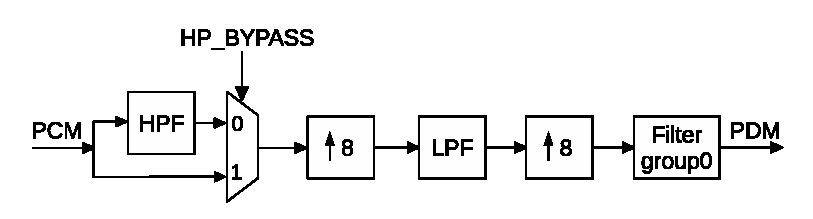
\includegraphics[width=0.6\textwidth]{./22-I2S/figures/i2s_pcm2pdm}}
    \caption{PDM 发送模块}
    \label{Figure:i2s_pcm2pdm}
\end{figure}

PDM 发送模块用于将 PCM 信号转换为 PDM 信号， 如图 \ref{Figure:i2s_pcm2pdm} 所示。HPF 为高通滤波器，LPF 为低通滤波器。PCM 信号经过上采样和滤波，最终输出 PDM 信号。寄存器 I2S\_PDM\_CONF\_REG 的 I2S\_TX\_PDM\_HP\_BYPASS 信号用于选择 PCM 信号是否经过 HPF 模块。Filter group0 模块具有上采样功能。假设 PDM 信号的频率为 $f_{\textrm{pdm}}$, PCM 信号的频率为 $f_{\textrm{pcm}}$, 那么 $f_{\textrm{pdm}}$ 与 $f_{\textrm{pcm}}$ 之间的关系为：
$$f_{\textrm{pdm}} = 64×f_{\textrm{pcm}}×\frac{ I2S\_TX\_PDM\_FP }{I2S\_TX\_PDM\_FS}$$
其中 64 为前面两次过采样率的乘积。

如表 \ref{table:过采样率配置} 所示，不同 PCM 信号的频率下，可以通过配置寄存器 I2S\_PDM\_FREQ\_CONF\_REG 的 I2S\_TX\_PDM\_FP 比特和 I2S\_TX\_PDM\_FS 比特， 得到输出频率均为 48×128 KHz 的 PDM 信号。

\begin{table}[H]
    \centering
    \caption{过采样率配置}
    \label{table:过采样率配置}
    \begin{tabular}{|p{3cm}|p{4.5cm}|p{4.5cm}|p{3cm}|}
    \hline
    \rowcolor{lightgray}
    $f_{\textrm{pcm}}$ (KHz)&I2S\_TX\_PDM\_FP & I2S\_TX\_PDM\_FS&$f_{\textrm{pdm}}$ (KHz)\\\hline
    48 	&960	&480&\multirow{6}*{48×128}\\
    \cline{1-3}
    44.1	&960	&441&\\
    \cline{1-3}
    32	&960	&320&\\
    \cline{1-3}
    24&960	&240&\\
    \cline{1-3}
    16	&960	&160&\\
    \cline{1-3}
    8	&960	&80 &\\
	\hline
    \end{tabular}
\end{table}

寄存器 I2S\_PDM\_CONF\_REG 的 I2S\_TX\_PDM\_SINC\_OSR2 比特表示 Filter group0 模块的过采样率。
$$I2S\_TX\_PDM\_SINC\_OSR2 = \left\lfloor\frac{I2S\_TX\_PDM\_FP }{I2S\_TX\_PDM\_FS}\right\rfloor$$


当使用 PDM 发送模块时，需要将寄存器 I2S\_PDM\_CONF\_REG 的 I2S\_TX\_PDM\_EN 比特与 I2S\_PCM2PDM\_CONV\_EN 比特全部置 1，如图 \ref{Figure:i2s_pdm_tx} 所示。寄存器 I2S\_PDM\_CONF\_REG 的 I2S\_TX\_PDM\_SIGMADELTA\_IN\_SHIFT 比特、I2S\_TX\_PDM\_SINC\_IN\_SHIFT 比特、I2S\_TX\_PDM\_LP\_IN\_SHIFT 比特和 I2S\_TX\_PDM\_HP\_IN\_SHIFT 比特用于调整各个滤波模块的输入信号的大小。

\begin{figure}[H]
    \centering
    \fbox{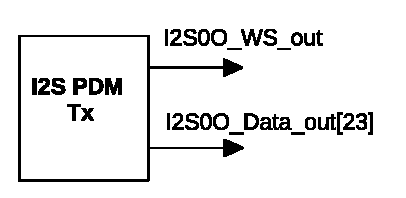
\includegraphics[width=0.35\textwidth]{./22-I2S/figures/i2s_pdm_tx}}
    \caption{PDM 发送信号}
    \label{Figure:i2s_pdm_tx}
\end{figure}

当使用 PDM 接收模块时，需要将寄存器 I2S\_PDM\_CONF\_REG 的 I2S\_RX\_PDM\_EN 比特与 I2S\_PDM2PCM\_CONV\_EN 比特全部置为 1，如图 \ref{Figure:i2s_pdm_rx} 所示。 PDM 接收模块结构将接收到的 PDM 信号转换为 16 比特的 PCM 信号。图 \ref{Figure:i2s_pdm2pcm} 中 Filter group1 用于对 PDM 信号进行下采样，寄存器 I2S\_PDM\_CONF\_REG 的 I2S\_RX\_PDM\_SINC\_DSR\_16\_EN 用于调整下采样率。PDM 接收模块的输入 PDM 信号频率需要为 PCM 信号 128 或 64 倍。

\begin{figure}[H]
    \centering
    \fbox{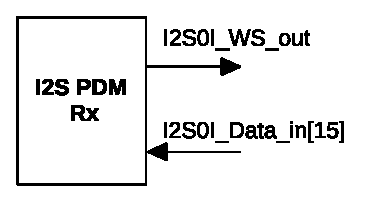
\includegraphics[width=0.35\textwidth]{./22-I2S/figures/i2s_pdm_rx}}
    \caption{PDM 接收信号}
    \label{Figure:i2s_pdm_rx}
\end{figure}

\begin{figure}[H]
    \centering
    \fbox{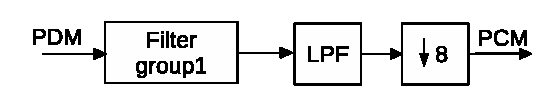
\includegraphics[width=0.5\textwidth]{./22-I2S/figures/i2s_pdm2pcm}}
    \caption{PDM 接收模块}
    \label{Figure:i2s_pdm2pcm}
\end{figure}


下表 \ref{table:下采样配置} 给出不同 PDM 信号的频率下，PDM 信号转 PCM 信号的 I2S\_RX\_PDM\_SINC\_DSR\_16\_EN 比特配置。

\begin{table}[H]
    \centering
    \caption{下采样配置}
    \label{table:下采样配置}
    \begin{tabular}{|p{4cm}|p{6cm}|p{5cm}|}
    \hline
    \rowcolor{lightgray}
    PDM freq (KHz)&I2S\_RX\_PDM\_SINC\_DSR\_16\_EN&PCM freq (KHz)\\
    \hline
     $f_{\textrm{pcm}}$×128&1&\multirow{2}*{$f_{\textrm{pcm}}$ }\\
    \cline{1-2}
    $f_{\textrm{pcm}}$×64&0&\\
    \hline
    \end{tabular}
\end{table}

\hypertarget{camlcdctrl}{}
\section{Camera-LCD 控制器}
\label{LCDMODE}
ESP32 I2S 的 LCD 模式分为：
\begin{itemize}
    \item LCD 主机发送模式
    \item Camera 从机接收模式
    \item ADC/DAC 模式
\end{itemize}
LCD 模式的时钟配置与 I2S 模式的时钟配置一致。LCD 模式下，WS 频率为 $f_{\textrm{BCK}}$ 的一半。

ADC/DAC 模式下，要使用 PLL\_F160M\_CLK 作为时钟源。

\subsection{LCD 主机发送模式}
如图 \ref{Figure:i2s_LCD} 所示，在 LCD 主机发送模式下，LCD 的 WR 信号接 I2S 模块的 WS 信号，数据信号线宽度为 24 比特。

\begin{figure}[H]
    \centering
    
\includegraphics[width=0.5\textwidth]{./22-I2S/figures/i2s_LCD}
    \caption{LCD 主机发送模式}
    \label{Figure:i2s_LCD}
\end{figure}

首先将寄存器 I2S\_CONF2\_REG 的 I2S\_LCD\_EN 比特置为 1，并且将寄存器 I2S\_CONF\_REG 的 I2S\_TX\_SLAVE\_MOD 比特置 0，使得 I2S 模块工作在 LCD 主机发送模式。同时，根据需要配置寄存器 I2S\_CONF\_CHAN\_REG 的 I2S\_TX\_CHAN\_MOD[2:0] 比特和寄存器 I2S\_FIFO\_CONF\_REG 的 I2S\_TX\_FIFO\_MOD[2:0] 比特，以使用正确的模式发送数据。WS 信号经过 GPIO 交换矩阵输出时需要反相。详情请参考章节 \hyperref[mod:intmtrx]{IO\_MUX 和 GPIO 交换矩阵}。在 LCD 模式主机发送模式下，还需要通过配置寄存器 I2S\_CONF2\_REG 的 I2S\_LCD\_TX\_SDX2\_EN 比特和 I2S\_LCD\_TX\_WRX2\_EN 比特，使得发送数据和 WR 信号工作在需要的模式下。

如图 \ref{Figure:i2s_lcd_frame_a} 和图 \ref{Figure:i2s_lcd_frame_b} 所示，数据帧格式 1 下，需要将 I2S\_LCD\_TX\_WRX2\_EN 比特置 1，I2S\_LCD\_TX\_SDX2\_EN 比特置 0 。 数据帧格式 2 下，需要将 I2S\_LCD\_TX\_SDX2\_EN 比特和 I2S\_LCD\_TX\_WRX2\_EN 比特都置 1。

\begin{figure}[H]
    \centering
    \fbox{
\includegraphics[width=0.6\textwidth]{./22-I2S/figures/i2s_lcd_frame_a}}
    \caption{LCD 主机发送数据帧格式 1}
    \label{Figure:i2s_lcd_frame_a}
\end{figure}

\begin{figure}[H]
    \centering
    \fbox{
\includegraphics[width=0.6\textwidth]{./22-I2S/figures/i2s_lcd_frame_b}}
    \caption{LCD 主机发送数据帧格式 2}
    \label{Figure:i2s_lcd_frame_b}
\end{figure}


\subsection{Camera 从机接收模式}

ESP32 I2S 可以配置成 Camera 从机模式，以此实现与外部 camera 模块的高速数据传输。在此模式下，I2S 模块为从机接收模式，除了 16 路数据信号总线 I2S\textcolor{red}{\it{n}}I\_Data\_in 外，还有 I2S\textcolor{red}{\it{n}}\_H\_SYNC、I2S\textcolor{red}{\it{n}}\_V\_SYNC和 I2S\textcolor{red}{\it{n}}\_H\_ENABLE 信号。

Camera 的 PCLK 接 I2S 模块的 I2S\textcolor{red}{\it{n}}I\_WS\_in 信号，如图 \ref{Figure:i2s_camera} 所示。
\begin{figure}[H]
    \centering
    
\includegraphics[width=0.5\textwidth]{./22-I2S/figures/i2s_camera}
    \caption{Camera 从机接收模式 }
    \label{Figure:i2s_camera}
\end{figure}

当 I2S 为 Camera 从机接收模式时，并且当 I2S\textcolor{red}{\it{n}}\_H\_SYNC、I2S\_V\_SYNC 和 I2S\_H\_REF 均为高电平时，认为主机开始传输数据，即：
$$transmission\_start= (  I2S\textcolor{red}{\it{n}}\_H\_SYNC==1) \&\& (  I2S\textcolor{red}{\it{n}}\_V\_SYNC==1 ) \&\& ( I2S\textcolor{red}{\it{n}}\_H\_ENABLE==1 ) $$
即在传输数据过程中，这三个信号需要保持高电平。例如某款 camera，I2S\textcolor{red}{\it{n}}\_V\_SYNC 信号在传输数据过程中为低电平，那么在输入 I2S 模块时 I2S\textcolor{red}{\it{n}}\_V\_SYNC 需要取反。ESP32 支持信号经过 GPIO 交换矩阵时取反。详情请参考章节 \hyperref[mod:intmtrx]{IO\_MUX 和 GPIO 交换矩阵}。

为了使 I2S 工作在 Camera 模式，寄存器 I2S\_CONF2\_REG 的 I2S\_LCD\_EN 比特和 I2S\_CAMERA\_EN 比特需要置为 1，并且将寄存器 I2S\_CONF\_REG 的 I2S\_RX\_SLAVE\_MOD 比特置 1， I2S\_RX\_MSB\_RIGHT 比特和\\I2S\_RX\_RIGHT\_FIRST 比特均设置为 0，使得 I2S 模块工作在 LCD 从机接收模式。同时，需要将寄存器\\I2S\_CONF\_CHAN\_REG 的 I2S\_RX\_CHAN\_MOD[2:0] 比特和寄存器 I2S\_FIFO\_CONF\_REG 的 I2S\_RX\_FIFO\_MOD[2:0] 比特均配置成 1，以使用正确的模式接收数据。

\subsection{ADC/DAC 模式}\label{sec:i2s-adc-dac}
LCD 模式使得片上 ADC 模块接收到的数据可以使用 I2S0 模块搬到内部存储区，也可以使用 I2S0 模块将内部存储区的数据搬到片上 DAC 模块。当 I2S0 模块连接片上 ADC 时，需要将 I2S0 模块配置为主机接收模式。图 \ref{Figure:i2s_adc} 为 I2S0 模块与 ADC 控制器之间的信号连接。

\begin{figure}[H]
    \centering
    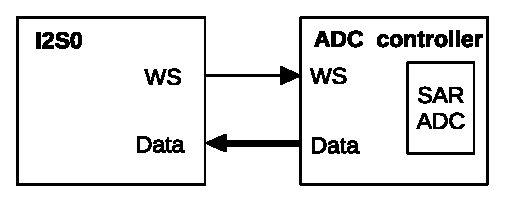
\includegraphics[width=0.45\textwidth]{./22-I2S/figures/i2s_sar_adc}
    \caption{I2S 的 ADC 接口}
    \label{Figure:i2s_adc}
\end{figure}

首先将寄存器 I2S\_CONF2\_REG 的 I2S\_LCD\_EN 比特置为 1，并且将寄存器 I2S\_CONF\_REG 的 I2S\_RX\_SLAVE\_MOD 比特置 0，使得 I2S0 模块工作在 LCD 主机接收模式，配置 I2S0 模块时钟，使得 I2S0 的 WS 信号输出合适的频率。然后将 SYSCON\_APB\_SARADC\_CTRL\_REG 寄存器的 SYSCON\_SARADC\_DATA\_TO\_I2S 比特置 1 。在配置好 SARADC 相关寄存器后启动 I2S 接收数据。详情请参考章节\hyperref[mod:sensor]{片上传感器与模拟信号处理}。

\begin{figure}[H]
    \centering
    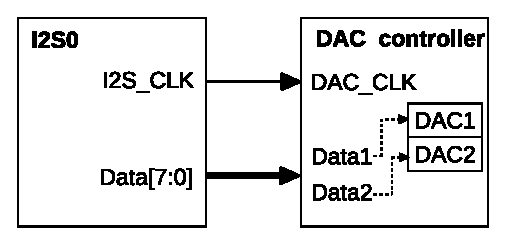
\includegraphics[width=0.45\textwidth]{./22-I2S/figures/i2s_dac}
    \caption{I2S 的 DAC 接口}
    \label{Figure:i2s_dac}
\end{figure}

\begin{figure}[H]
    \centering
    \fbox{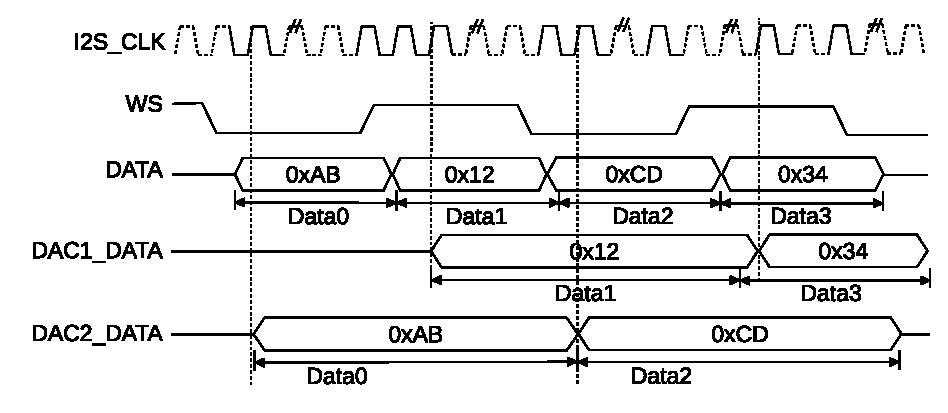
\includegraphics[width=0.7\textwidth]{./22-I2S/figures/i2s_dac_data}}
    \caption{I2S DAC 接口数据输入}
    \label{Figure:i2s_dac_data}
\end{figure}

当 I2S0 模块接片内 DAC 时，需要将 I2S0 模块配置成主机发送模式。图 \ref{Figure:i2s_dac} 为 I2S0 模块与 DAC 控制器之间的信号连接。DAC 控制模块以 I2S\_CLK 为时钟，此时 I2S\_CLK 最高为 APB\_CLK/2。如图 \ref{Figure:i2s_dac_data} 所示，当数据总线向 DAC 控制模块输入数据时，DAC 控制器会将右声道数据输入 DAC1 模块，将左声道数据输入 DAC2 模块。使用 I2S DMA 模块时， 需要将待发送的 8 位数据左移 8 位填入 DMA 的双字节类型 buffer 中。

使用 I2S0 的 DAC 模式时，首先将寄存器 I2S\_CONF2\_REG 的 I2S\_LCD\_EN 比特置为 1，分别将 I2S\_RX\_SHORT\_SYNC、I2S\_TX\_SHORT\_SYNC、I2S\_CONF\_REG、I2S\_RX\_MSB\_SHIFT 和 I2S\_TX\_MSB\_SHIFT 清零，并且将寄存器\\I2S\_CONF\_REG 的 I2S\_TX\_SLAVE\_MOD 比特置 0，使得 I2S0 模块工作在 LCD 主机发送模式。按照传输 16 位数据的标准， 选择合适的发送模式。 配置 I2S0 模块时钟，使得 I2S 的 I2S\_CLK 和 WS 输出合适的频率。 在配置好 DAC 相关寄存器后，启动 I2S0 发送数据。

\section{I2S 中断}
\subsection{FIFO 中断}

\begin{itemize}
\item \label{int:I2STXHUNGINT}I2S\_TX\_HUNG\_INT：当发送数据超时即触发此中断。
\item \label{int:I2SRXHUNGINT}I2S\_RX\_HUNG\_INT：当接收数据超时即触发此中断。
\item \label{int:I2STXREMPTYINT}I2S\_TX\_REMPTY\_INT：当发送 FIFO 为空时即触发此中断。
\item \label{int:I2STXWFULLINT}I2S\_TX\_WFULL\_INT：当发送 FIFO 满时即触发此中断。
\item \label{int:I2SRXREMPTYINT}I2S\_RX\_REMPTY\_INT：当接收 FIFO 为空时即触发此中断。
\item \label{int:I2SRXWFULLINT}I2S\_RX\_WFULL\_INT：当接收 FIFO 满时即触发此中断。
\item \label{int:I2STXPUTDATAINT}I2S\_TX\_PUT\_DATA\_INT：当发送 FIFO 将要空时即触发此中断。
\item \label{int:I2SRXTAKEDATAINT}I2S\_RX\_TAKE\_DATA\_INT：当接收 FIFO 将要满时即触发此中断。
\end{itemize}

\subsection{DMA 中断}\label{DMA Interrupts}
\begin{itemize}
\item \label{int:I2SOUTTOTALEOFINT}I2S\_OUT\_TOTAL\_EOF\_INT：当所有发送链表使用完毕时即触发此中断。
\item \label{int:I2SINDSCREMPTYINT}I2S\_IN\_DSCR\_EMPTY\_INT：无有效接收链表可用时即触发此中断。
\item \label{int:I2SOUTDSCRERRINT}I2S\_OUT\_DSCR\_ERR\_INT：当遇到无效发送链表描述符时即触发此中断。
\item \label{int:I2SINDSCRERRINT}I2S\_IN\_DSCR\_ERR\_INT：当遇到无效接收链表描述符时即触发此中断。
\item \label{int:I2SOUTEOFINT}I2S\_OUT\_EOF\_INT：当发送链表完成发送一个数据包时即触发此中断。
\item \label{int:I2SOUTDONEINT}I2S\_OUT\_DONE\_INT：当所有发送缓存数据被读取完毕后即触发此中断。
\item \label{int:I2SINSUCEOFINT}I2S\_IN\_SUC\_EOF\_INT：当所有数据接收完毕时即触发此中断。
\item \label{int:I2SINDONEINT}I2S\_IN\_DONE\_INT：当前接收链表描述符被处理时即触发此中断。
\end{itemize}

\hypertarget{i2s-reg-summ}{}
\section{寄存器列表}\label{sec:i2s-reg-summ}

本小节的所有地址均为相对于 I2S 基地址的地址偏移量（相对地址），具体基地址请见章节 \ref{mod:sysmem} \textit{\nameref{mod:sysmem}} 中的表 \ref{table:Peripheral_Address_Mapping}。

请查看章节 \hyperref[glossary-access-types]{\textit{寄存器的访问类型}}，了解“访问”列缩写的含义。

\subfile{\modulefiles/i2s_reg-summary_cn.tex}
{\clearpage}

\section{寄存器}\label{I2SRegister}

本小节的所有地址均为相对于 I2S 基地址的地址偏移量（相对地址），具体基地址请见章节 \ref{mod:sysmem} \textit{\nameref{mod:sysmem}} 中的表 \ref{table:Peripheral_Address_Mapping}。寄存器绝对地址见章节 \ref{sec:i2s-reg-summ} \textit{\nameref{sec:i2s-reg-summ}}。

关于保留 (reserved) 域的处理，请查看章节 \hyperref[programming-reserved-field]{\textit{如何配置寄存器的保留域}}。


\subfile{\modulefiles/i2s_reg_cn.tex}
\end{document}
